

\chapter{Úvod}





\chapter{Java Enterprise edition 6}
V posledných rokoch prevláda tendencia tvorby komplexných informačných systémov, ktoré spracovávajú veľké množstvo dát. Preto sa zvyšuje tlak na vývojárov na tvorbu prostriedkov, ktoré dokáže takéto systémy ľahko a rýchlo vytvárať. Jedným z takýchto protriedkov je platforma Java Enterprise Edittion 6(Java EE 6).
Java EE 6 predstavuje platformu určenú na vývoj webových a podnikových aplikácií.\cite{fitWeb}Tieto aplikácie sú viacvrstvové z dôvodu lepšej prenositeľnosti, nasaditeľnosti a modifikovateľnosti. Frontend, predstavujúci užívateľské rozhranie a logiku na jeho ovládanie, pozostáva z webových frameworkov, stredná vrsta poskytuje bezpečnosť a transakcie. Najnižšia vrstva poskytuje pripojenie k databázam. Java EE 6 je vhodná pre implementáciu podnikovej logiky, ktorá dokáže byť riadená alebo interagovať s inými podnikovými aplikáciami. Java EE 6 je platformou, ktorá poskytuje širokú škálu aplikačných programových rozhraní(API), ktoré zjednodušujú, zkracujú a znižujú komplexnosť výslednej aplikácie. Jej vývoj neustále napreduje a je spravovaný Java Comunnity process(JCP).


\indent Java EE 6 bola uvoľnená v decembri 2009 a poskytuje ľahké používanie a kompletnú sadu nástrojov na tvorbu podnikových aplikácií. V súčastnosti vyšla ďalšia verzia, ktorá priniesla ďalšie novinky, ktoré môžte dohľadať v online dokumentácií. V ďalších kapitolách si rozoberieme aplikaný model jazyka, ktoré je veľmi dôležitý pre pochopenie princípu činnosti aplikácií vyvinutých touto platformou. V ďalšej kapitole rozobereme aplikačný model platformy Java EE 6. 


\section{Aplikačný model}
Java EE je určená pre implementáciu služieb pre zákazníkov, zamestnancov, dodávateľov kohokoľvek, kto prispieva do podniku. Takéto aplikácie sú komplexné a môže byť k nim pristupované z rozličných zdrojov. Pre lepšie zvládanie sú sústredené do stupňov.

\indent Java EE definuje spôsob implementácie služieb, ktoré sú škálovateľné a prístupné.

\section{Distribuovaná viacstupňová aplikácia}
Java EE definuje aplikácie, ktoré sú viacvrstvové(multitier). Aplikačná logika je rozdelená medzi komponenty podľa ich funkcie.\cite{Pravidla} Jednotlivé komponenty sa následne rôzne inštalujú v závislosti, do ktorého stupňa patria. Jednotlivé stupňe sa skladajú z rôznych komponent:
\begin{itemize}
\item Klientská komponenta, ktorá beží na klientskom počítači
\item Webová komponenta, ktorá beží na Java EE serveri
\item Podniková komponentna, ktorá beží na Java EE serveri
\item Enterprise Information System software bežiaci na EIS serveri
\end{itemize}

Napriek tomúto rozloženiu býva aplikácia rozložená len do 3 stupňov: Java EE server, klient, databáze. Typicky beží medzi klientskom a databázou častou viac-vláknový Java EE server, ktorý býva označovaný skratkou EIS. Viacstupňovérozloženie môžete názorne vidieť na obrázku č. \ref{model}.
\begin{figure}[htb]

\begin{center}

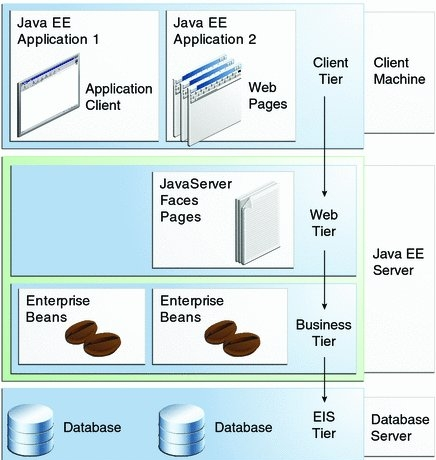
\includegraphics[scale=0.5]{model.jpg} 
\caption{Model Java EE, prevzaté z  http://docs.oracle.com/javaee/6/tutorial/doc/}
\label{model}

\end{center}

\end{figure}
Java EE aplikácia beží na klientskej stanici, býva obykle reprezentovaná tenkým klientom(webovým prehliadačom), nazývaným \uv{thin client}, alebo hrubým klientom, do ktoré je čiastočne vložená logika aplikácia. V strednej časti obrázku sa nachádza Java EE server, na ktorom môžu bežať rôzne technológie v závislosti od požiadavky výslednej aplikácie a možností daného servera. Java EE server môže by reprezentovaný rôznymi dostupnými technológiami, či už sa jedná o open-source riešenia (JBoss, Tomcat, GlassFish) alebo komerčné riešenia (IBM WebSphere,BEA WebLogic), ten obsahuje rôzne komponenty, ktoré so sebou rôzne komunikujú a interagujú na požiadavky klienta a na druhej strane komunikujú s databázovým systémom. Tieto komponenty predstavujú logiku aplikáciu. Posledná časť predstavuje databázový systém, ktorý obsahuju dáta, ktoré klient požaduje pri svojom požiadavku, tento server sa nazýva "EIS".

\section{Bezpečnosť}

Java EE  vytvára prostriedky, ktoré sú prenositeľné a tak je možné systémy nasadzovať naprieč rôznymi platformami. Poskytuje mechanizmus  prístupovej kontroly pravidiel, ktoré sú interpretované, keď je aplikácia nasadzovaná na server. Java implementuje mechanizmus prihlasovania štandardne, čím odpadá programátori povinnosti túto časť dodatočne implementovať.

V ďalšej časti sa zameriame na podrobné vysvetlenie jednotlivých Java EE komponent, pretože ich pochopenie bude nevyhnuté pre výslednú aplikáciu.


\section{Java EE komponenty}
Java EE pozostáva z komponent, čo je vlastne sada sebestačného softwaru, ktorý je zhromaždený do Java EE aplikácií a komunikujú s inými komponentami. Java EE definuje nasledujúce komponenty: 
\begin{itemize}
\item Aplikačný klienti a aplety bežiaci na klientovi
\item Java Servlet, JavaServer Faces, and JavaServer Pages (JSP) komponenty bežia na Java EE serveri\cite{fitWeb}.
\item Enterprise JavaBeans (EJB) komponenty bežia na Java EE serveri\cite{fitWeb}.
\end{itemize}

V nasledujúcej časti sa zameriami na vysvetlenie jednotlivých pojmov, pretože sú doôležité z hľadiska pochopiteľnosti výslednej aplikácie.

\section{Java EE klienti}
Java EE client je typicky webový klient alebo aplikačný klient.

Typický webový klient pozostáva z dvoch častí:
\begin{itemize}
\item Dynamické webové stránky pozostávajúce z rôzneho značkovacieho jazyka(HTML, XML), ktoré sú generované webovými komponentami
\item Webovým prehliadačom, ktorý zobrazuje stránky
\end{itemize}
Typický webový klient sa nazýva "thin" klient, pretože nedotazuje nad databázou, alebo implementuje zložitú bussiness logiku. Všetky tieto činnosti vykonavá Java EE server. Klient len posiela požiadavky Java EE serveru a ten vykonáva dotazovanie a predávanie výsledkov.


Aplikační klienti bežia na klientských počítačoch, kde poskytujú bohatšie užívateľské rozhranie ako webový rozhrania značkovacích jazykov.
Typicky býva vytváraný technológiou Swing\footnote{http://cs.wikipedia.org/wiki/Swing\_(Java)} alebo Abstract Window Toolkit(AWT)\footnote{http://en.wikipedia.org/wiki/Abstract\_Window\_Toolkit}, občas sa vyskytuje aj prikázový riadok ako rozhranie.

\section{The JavaBeans Component Architecture}
Server a klient tiež zahŕňa komponenty založené na JavaBeans component architecture(JavaBeans components), ktoré správujú toky dát medzi:
\begin{itemize}
\item Aplikačným klientom,alebo apletom a komponentami bežiacimi na Java EE serveri
\item Serverovými komponentami a databázami
\end{itemize}


Komunikácia medzi klientom s podnikovým stupňom, ktorý sa nachádza na Java EE serveri, v prípade, že klient beží v prehliadači.

\section{Webové komponenty}
Java EE webové komponenty sú súčasťou servletov alebo webových stránok, ktoré sú vytvorené JavaServer Faces technológiu(JSF) and JavaServer pages(JSP) technológiou.
Servlety sú javovské triedy , ktoré dynamicky spracovávajú požiadavky a tvoria odpovede. JSP stránky sú textové dokumenty, ktoré pracúvajú ako servlety ale umožňujú prirodzenejší prístup k vytváraniu statického obsahu. JavaServer Faces technológia stavia na servlety a JSP technológie a poskytuje užívateľské rozhranie komponentný framework pre webové aplikácie.


\subsection{Java Persistence API}
Java Persistence API(JPA) je špecifikácia jazyku Java, ktorý poskytuje objektovo relačné mapovanie. Java Persistence API využíva pre mapovanie entity, ktoré reprezentujú dáta v databázi. Typicky teda reprezentuju tabuľku databáze a jej každá inštacia riadok tabuľky. Entitná trieda má teda atribúty, ktoré priamo odpovedajú názvu stĺpcov v databázovej schéme. To značne uľahčuje a zprehľadňuje prácu s databázou. Pre prístup k databáze sa používa trieda EntityManager, ktorá spracováva transakcie a zabezpečuje aby boli spĺňali podmienky ACID. Java Persistence API rovnako definuje vlastný jazyk Java Persistence Query Language, čo je jazyk podobný jazyku SQL, ktorý využíva trieda EntityManager pri svojej práci. Výhodou je, že tento jazyk je nezávislý na zvolenej databázovej technológií a má objektové vlastnosti, teda pri dotazoch nepoužívame konkrétne názvy tabuliek ale názvy entitný tried a jej vlastností. 

Medzi konkrétne implementácie JPA patrí: Hibernate, Oracle TopLink, OpenJPA.

\subsection{Enterprise Bean}
Enterprise Bean(WB) sú Java EE komponenty, ktoré implementujú Enterprise JavaBeans(EJB) technológie. Enterprise bean beží v kontajneri EJB. EB je server-side komponentov, ktorá zapuzdruje enterprise logiku aplikácie. Obchodná logika je kód, ktorý spĺňa účel použitia. Z niekoľkých dôvodov, EB zjednodušuhe vývoj rozsiahlych, distribuovaných aplikácií. Po prvé, pretože kontajner EJB poskytuje služby na úrovni systému a vývojár sa môže sústrediť na riešenie obchodných problémov. Kontajner EJB, je zodpovedný za služby na úrovni systému, ako je riadenie transakcií a autorizácie zabezpečenia.


EB sa delia na 2 kategórie:
\begin{itemize}
\item Message-driven - Vykoná úloha pre klienta; voliteľne môže implementovať webové služby
\item Session - Pôsobí ako poslucháča pre určitý typ správ, ako je API Java Message Service

\end{itemize}



\section{JavaServer Faces}
JavaServer Faces zodpovedá serverovej strane frameworku pre užívatelské rozhrania vychádzajúce z Javy. JavaServer Faces(JSF) vytvára aplikácie na základe MVC - Model-View Controller. Ďalej treba spomenúť, že pomáha previazať užívatelské údaje so serverom, rovnako ako aj komponenty, ktoré sú znova použitelné.

\indent Aplikácia, ktorá je vytvára týmto frameworkom pozostáva z webových stránok, grafických komponent, sadou komponent naviazané na serverovú časť. Môže obsahovať rôzne desktriptory a konfiguračné súbory, ktoré nám pomáhujú pri nasadzovaní aplikácie. Základom JavaServer Faces je Facelets, čo je vlastne výzorovo deklaračný jazyk pre JSF. Facelets stránky používajú XHTML 1 a CSS. 


V ďalšej časti sa zameriame na JBoss a OptaPlanner.

\section{Web Service}
Web Service  sú klientské a serverové aplikácie, ktoré komunikujú prostredníctvom HTTP protokolu vymenieňaním XML správ. Tieto aplikácie poskystujú interoperabilitu medzi rôznymi platformami naprieč počítačou sieťou. Web Service umožňuje komunikáciu medzi rôznymi aplikáciami, ktoré bežia na rôznych platformách, napr. Java aplikácie založené na Windowse komunikujú s Net. aplikácia bežiaci na Linuxe. Webo services  sa delia na 2 kategórie "big" web services a "RESTFul" web services.

\subsection{"Big" Web Services}
V Jave EE 6 existuje API, ktoré sa nazýva JAX-WS, ktoré umožňuje vytvorenie práve tohto typu web servici.\cite{fitWeb} "Big" web service využíva XML správy, spolu so SOAP a XML jazykom, ktorý definuje architekrúru a formát správ. Tento typ Web Service obsahuje definíciu pre Web Service vo formáte WSDL, ktorý je čitatelný aj počítačom. Formát SOAP správ a definíciu jazyka WSDL rozhrania môže znížiť zložitosť vývoja aplikácií, webových služieb. 

\subsection{RESTful Web Service}
V Java EE 6 existuje pre druhý typ web service API, ktoré sa nazýva JAX - RS. Tento typ web serrvice je vhodný pre základné , ad hoc integračné scenáre. REST webové služby, často lepšie integrované s HTTP ako službami založenými na SOAP je , nevyžadujú XML správ alebo definície WSDL služby - API.


\subsection{Iné technológie}
\subsubsection{Maven}
Maven  je založený na centrálnej konceptu životného cyklu zostavenie. Čo to znamená, že proces budovania a distribúciu určitého artefaktu(projektu) je jasne definovaná. Depency management je jedným z rysov Maven-u, ktorý je najlepšie známy pre užívateľa a je jednou z oblastí, kde Maven vyniká. Maven sa používa hlavne pre multimodulové aplikácie pre zachovanie vysokého stupňa kontroly a stability.

Životný cyklus pozostáva z fáz. Každá z týchto zostavenie životný cyklus je definovaný iným zoznamu zostavenie fáz, pričom fáza zostavenie predstavuje fázu životného cyklu. Maven môže generovať dokumentáciu projektu a  vytvoriť stavbu. Maven má niekoľko správ, ktoré sa môžu pridať na webové stránky a zobraziť aktuálny stav projektu. Tieto správy majú formu pluginov, rovnako ako tie používané na zostavenie projektu.

Internacionalizácia v Maven je veľmi jednoduché.\cite{mavenbook}

\subsubsection{Arquillian}
Arquillian je integračne a funkčne testovacia platforma, ktorá môže byť použitá pre testovanie middleware Java. Jej hlavným cieľom je urobiť integráčné(a funkčné) testy tak jednoduché písať unit testy, čo umožňuje vývojárom riadenie behu v rámci testu. 
Arquillian podporuje integráciu s Java EE kontajnermi, ako je JBoss AS a GlassFish a servlet kontajnerov, ako sú Tomcat a Jetty, a podporuje vykonávanie testov v cloudových službách. Podpora kontajnerov umožňuje vývojárom zamerať sa na rad technologických platforiem, vrátane Java EE 5 a 6, servlet prostredie, OSGI, Embedded EJB a samostatné CDI.\cite{arqbook}


\chapter{JBoss Aplication Server} 
JBoss, čo je vlastne skratka pre JavaBeans Open Source Applicatom Server, v súčastní nazývaný WildFly je aplikačný server, ktorý je založený na platforme Java a Java Enterprise Edition.\cite{jbossbook} Aplikačný server tvorí vrstvu medzi aplikáciami a operačným systémom, pričom rovnako poskytuje aplikácia často využívané funkcie, napr. spracovanie transakcií, výmená správ, \ldots . Aplikačné servery podobne ako JBoss Aplication Server(JBoss AS) je open source. JBoss je Java EE platforma pre vývoj a nasadzovanie Java aplikáciu, webových aplikácií, služieb a portálov.

 JBoss AS je napísaný v Jave, preto existuje možnosť  ho používať naprieč rôznym platformám. Tento server slúži na vývoj a nasadzovanie podnikových aplikácií, webových aplikácií, služieb a portálov. Tento server je licensovaný pod GNU Lesser General Public License(GNU PL).

\section{História JBoos-u}
Všetko naštartoval v roku 1999 Marc Fleury. Pre podporu vývoja middleware InterBohemia sebe rozhodol implementovať jeden zo štandardov J2EE , EJB kontajner. Tým sa zrodil prvý projekt - EJBoss, ktorý sa neskôr premenoval na JBoss. TO niekoľko rokov neskôr sa stal prvým certifikovaným  J2EE  open source aplikačným serverom. Ďalej by som rád ukázal na vývoj rôznych verzií JBossu:\cite{jbossWeb}


\begin{itemize}
\item JBoss AS 4.0 , Java EE aplikačný server 1.4, je vybavený vloženým Apache Tomcat 5.5 servlet kontajnerom. JBoss môže bežať na mnohých operačných systémoch, vrátane mnohých POSIX platformách (ako GNU/Linux , FreeBSD a Mac OS X) , Microsoft Windows a ďalšie
\item JBoss AS 5.1 , povolený v roku 2009, pracuje ako Java EE 5 aplikačný server. Je to menšia aktualizácia hlavnej verzie JBoss AS 5.0, ktorý bol vo vývoji po dobu najmenej troch rokov a bol postavený na vrchole novej JBoss microcontainer.

\item JBoss AS 6.0, bol neoficiálne implementáciou Java EE 6, vydané 28. decembra 2010 .

\item JBoss AS 7, bola vydané 12. júla 2011, len šesť mesiacov po poslednej hlavnej verzie , JBoss AS 6. JBoss AS 7 podporuje rovnaké špecifikáciu Java EE ako posledná verzia, a to Java EE 6. Java EE profil je iba čiastočne implementovaný v JBoss AS 7. Hlavné zmeny viditeľné pre užívateľa sú: oveľa menšiu veľkosť ( menej než polovica z JBoss AS 6 ) a násobné zníženie v čase spustenia.

\item JBoss AS 7. , aktuálna stabilná verzia bola vydaná vo februári 2012 . Zostávajúce časti EE špecifikácie boli realizované , a táto verzia bola certifikovaná pre EE plnom profile.

\item WildFly 8 je priamym pokračovaním na JBoss AS projektu .

\end{itemize}

V ďalšej časti sa zameriame na OptaPlanner, čo je vlastne systém, pre ktorý je rozhranie navrhované.




\chapter{OptaPlanner}
OptaPlanner je odľahčený open source software a ďalšie prokračovanie frameworku JBoss Drools, ktorý optimalizuje plánovacie problémy.\cite{optaweb} Tieto plánovacie problémy môžu byť nasledujúceho charakteru: 
\begin{itemize}
\item Plánovanie agendy: plánovanie schôdzok, vymenovanie, práca údržby
\item Plánovanie vzdelávania: plánovanie lekcie, kurzov
\end{itemize}
\begin{figure}[htb]

\begin{center}

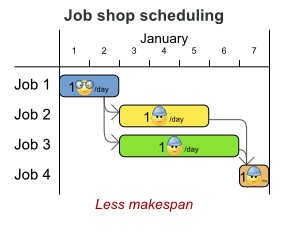
\includegraphics[scale=0.5]{fig/useCaseOverview.jpg} 
\caption{Job, Shop scheluding, prevzaté z http://www.optaplanner.org/ }
\label{obrazokUseCase}

\end{center}

\end{figure}
Obrázok č. \ref{obrazokUseCase} zobrazuje typické použitie OptaPlanner-u. Môžme vidieť v nasledujúcom obrázku vystupú 4 osoby, ktoré vykonávajú nejakú činnosť. Ich činnosť je špecifická a silne závisí od práce predchádzajúcich. Optaplanner sa snaží ich činnosti maximálne optimalizovať a jednotlivé činnosti zvoliť v následnosti tak, aby výsledná práca bola spravená za najkratší možný čas vzhľadom na činnosť, ktorá sa optimalizuje.


\subsection{NP-úplný problém}
Každý plánovací problém je NP-úplný problém.\cite{npbook} NP-úplné problémy sú nedeterministicky polynomiálne problémny, ktoré nie sú riešitelné v dostupnom čase, pretože sa nepodarilo nájsť deterministický algoritmus. Príkladom NP úloh môžme považovať: problém obchodné cestujúceho, \ldots .

Riešenia poskytnutým týmto frameworkom, ktorý využíva pokročilé optimalizačné algoritmy, sú dosiahnuteľné v reálnom čase. Dosiahnutie v reálnom čase znamená nájdenie 1 alebo viacerých riešení, alebo nenájdenie žiadneho riešenia vzhľadom na poskytnutý čas a optimalizačné algoritmy, ktoré sú implementované.

Každý plánovací problém je definovaný na základe obmedzení, ktoré musia minimálne spĺnať: \cite{optabook}
\begin{itemize}
\item Negatívne "hard" obmedzenie, ktoré nesmie byť porušené
\item Negatívne "soft" obmedzenie, ktoré by nemali byť porušené pokiaľ sa dá tomu vyhnúť.
\end{itemize}

Niektoré problémy môžu obsahovať aj pozitívne podmienky alebo odmeny, ktoré by mali byť splnené pokiaľ je možné ich splniť.

Tieto podmienky definujú skóre plánovacieho problému. Tieto podmienky môžu byť zapísané v Jave alebo v Drools pravidlách, ktoré značne zjednodušujú kód.

 Vytvorenie je pomocou pravidiel  môže robiť  oveľa jednoduchšie spájať mnoho pravidiel s mnohými akciami. Tieto pravidlá bývajú typicky definované pomocou XML súboru.

OptaPlanner pomáha  programátori riešiť obmedzenie problémov spokojnosti efektívne. Pod kapotou sa kombinuje optimalizačné heuristiky na výpočet skóre.



\subsection{Výsledky plánovacieho problému}

Tieto obmedzenia definujú výpočetné skóre problému plánovania. Každé riešenie problému plánovanie môže byť odstupňovaná so skóre. 

Plánovanie problému má niekoľko riešení. Existuje niekoľko kategórií riešení:
\begin{itemize}
\item Možným riešením je nejaké riešenie, či je alebo nie je ľubovoľný počet obmedzení. Problémy plánovanie mávajú neuveriteľne veľké množstvo možných riešení. Mnoho z týchto riešení sú bezcenné.
\item Uskutočniteľným riešením je riešenie, ktoré neporušuje žiadne (negatívne) tvrdé obmedzenia. Niekedy nie sú realizovateľné riešenie. Každý uskutočniteľné riešenie je možné riešenie.

\item Optimálnym riešením je riešenie s najvyšším počtom bodov. Problémy plánovanie mávajú jedno alebo niekoľko optimálnych riešení. K dispozícii je vždy aspoň 1 optimálnym riešením, a to aj v prípade , že neexistujú žiadne uskutočniteľné riešenie, a optimálne riešenie nie je možné .
\item Najlepším riešením je nájsť riešenie s najvyšším skóre zistené implementáciou v danom čase.

\end{itemize}

OptaPlanner podporuje niekoľko optimalizačných algoritmov ako efektívne prehrýzť týmto neuveriteľne veľkým množstvom možných riešení. V závislosti na prípade použitia, niektoré optimalizačné algoritmy dosahujú lepšie výsledky ako ostatné, ale to je nemožné povedať dopredu. Pri plánovaní , je ľahké prepnúť algoritmus optimalizácie, zmenou konfigurácie Solver na niekoľkých riadkov XML alebo kódu.


\newpage
\subsection{Ukážka XML configuračného súboru}
V nasledujúcom obrázku by som rád ukázal príklad XML configuračného súboru pre OptaPlanner.
 \lstset{
    language=xml,
    tabsize=3,
    %frame=lines,
    caption=Test,
    label=code:sample,
    frame=shadowbox,
    rulesepcolor=\color{gray},
    xleftmargin=20pt,
    framexleftmargin=15pt,
    keywordstyle=\color{blue}\bf,
    commentstyle=\color{OliveGreen},
    stringstyle=\color{red},
    numbers=left,
    numberstyle=\tiny,
    numbersep=5pt,
    breaklines=true,
    showstringspaces=false,
    basicstyle=\footnotesize,
    emph={food,name,price},emphstyle={\color{magenta}}}
    \lstinputlisting{cloudBalancingSolverConfig.xml}

\newpage
Konfigurácie solveru pozostáva z 3 častí: 
\begin{itemize}
\item Domail model configuration: Musíme Optaplanneru uviesť hlávnú triedu.
\item Configurácia skóre, ktorá hovorí Optaplanneru ako ma optimalizovať premenné. Pokiaľ používame hard a soft obmedzenia, použijeme "HardSoftScore". Musíme tiež uviesť ako vypočítať také skóre, v závislosti na našich požiadavkách. Ďalej sa, sme musíme  pozrieť do 2 alternatívy pre výpočet skóre: pomocou jednoduchej implementácie Java, alebo pomocou Drols DRL.Optaplanner bude hľadať riešenie s najvyšším skóre. Budeme používať HardSoftScore, čo znamená, plánovač bude hľadať riešenie s žiadnymi tvrdými obmedzeniami členenie (spĺňajú požiadavky na hardvér) a pokiaľ možno čo najmenej mäkkých obmedzenia členenie (minimalizovať náklady na údržbu).
\item Konfigurácia optimalizačných algoritmov

\end{itemize}

\subsection{Optimalizačné algoritmy}
V nasledujúcej časti textu si ukážeme optimalizačné algoritmy, ktoré používa optaplanner.
\begin{itemize}
\item First FIT - To je veľmi jednoduché greedy algoritmus aproximácie. Algoritmus spracováva položky v ľubovoľnom poradí. Pre každú položku, pokúsi sa umiestniť na položku v prvej priehradke, ktorý sa môže ubytovať položku. Ak nie je nájdený žiadna priehradka, otvára novú priehradku a kladie položku v rámci nového zásobníka.

\item Firt FIT Decreasing
\item Firt FIT Decreasing + heurestic local search

\begin{itemize}
\item Hill Climbing - hill climbing je matematická optimalizácia technika, ktorá patrí do rodiny miestneho vyhľadávania. Jedná sa o iteratívny algoritmus, ktorý začína s ľubovoľným riešenie problému, potom sa pokúsi nájsť lepšie riešenie tým, že postupne mení jeden prvok riešenia. Ak zmena vytvára lepšie riešenie zmeny sa opakujú až žiadne ďalšie zlepšenie nie je možno nájsť.\cite{algobook}




\item Tabu Search - Tabu search používa miestny alebo susedcký postup vyhľadávanie, tak že iteratívne presuvá z jedného možného riešenia x k lepšiemu riešeniu x  v susedstve x, kým sa niektoré kritérium zastavenia splní. Miestne postupy vyhľadávania sa často uviaznu v zle bodovaných oblastiach. V snahe vyhnúť sa týmto nástrahám a preskúmať oblasti hľadaného miesta, ktoré by mali zostať bez prehliadky inými miestnymi postupmi vyhľadávania, tabu search starostlivo skúma okolí každého toku ako hľadanie postupuje. Riešenie prijatí do novej štvrti  sú určené pomocou pamäťových štruktúr.

\item Simulated Annealing - Simulované žíhanie je všeobecný algoritmus pre globálne optimalizačné problémy lokalizovať dobré priblíženie k globálnej optimálnej danej funkcie vo veľkom vyhľadávacieho priestoru. To sa často používa pri hľadaní priestorov diskrétnych (napr. všetky výlety, ktoré navštevujú danú množinu miest). U niektorých problémov, môže simulované žíhanie byť účinnejšie ako vyčerpávajúci zoznam - za predpokladu, že cieľom je iba nájsť prijateľne dobré riešenie v stanovenú dobu, skôr ako tým najlepším možným riešením .

\end{itemize}

\end{itemize}


V ďalšej kapitole by som rád uviedol problematiku užívateľského rozhrania.
\chapter{Grafické užívateľské rozhranie}
V tejto kapitole sa zameráme na problematiku užívateľského rozhrania, ktoré vlastne je reprezentované prostredíctvom technológie Java Server Faces v kombinácií frameworkov Rich Faces a Twitter Bootstrap-u. Toto rozhranie bude umožňovať nahrávať pravidlá, zobrazovať výsledky, spúšťať, pozastovať a zobrazovať detaily úloh. Keďže táto výsledná aplikácia by mala byť použíteľná aj na mobilnom telefóne bol vybratý štýlovací framework Twitter Bootstrap, ktorý značne uľahčenie tvorbu takéhoto rozhrania.

\section{Twitter Bootstrap}
Twitter Bootstrapje veľmi jednoduchý a voľne dostupný súbor nástrojov pre vytváranie moderného webu a webových aplikácií.\cite{boot} Ponúka podporu najrôznejších webových technológií HTML , CSS , JavaScript a mnoho prvkov , ktoré je možné ľahko implementovať do svojej stránky. Pre použitie Twitter Bootstrap sú nutné základné znalosti HTML a CSS. Interaktívne prvky ako sú tlačidlá, boxy , menu a ďalšie kompletne nastavené a graficky spracované elementy je možné vložiť iba pomocou HTML a CSS .

Výhodou tohto súboru nástrojov je jednoduché spracovanie akéhokoľvek používateľského rozhrania vo webovej aplikácii a nerozhoduje , či to je napríklad používateľské rozhranie v administrácii back-endových alebo front-endových aplikácií.


Podrobné vysvetlenie jednotlivých komponent nájdete na nasledujúcej adrese http://getbootstrap.com/, rovnako aj s príkladmi použitia. V nasledujúcej časti prejdem na samotný návrh užívateľského rozhrania.

\section{Rich Faces}
Rich faces predstavuje open-source Ajax knižnicu, ktorá predstavuje rozšírenie pre JavaServer Faces. Umožňuje integráciu schopností ajaxu do enterprise aplikácií. RichFaces obohacuje framework Ajax4jsf v dvoch dôležitých ohľadoch. Po prvé, sa rozširuje množstvo vizuálnych pripravených komponent. Po druhé,  plne implementuje funkciu skinnability rámca Ajax4jsf vrátane veľkého množstva preddefinovaných vzhľadov. Pomocou skinnability, že je oveľa ľahšie riadiť vzhľad aplikácie.


\section{Rozbor aplikácie}
Výsledná aplikácia bude zobrazovať priebežné výsledky výpočtu frameworku optaplanner. Tento framework bude pre túto prácu optimalizovaný pre úlohu N Dám, ktorú bude schopný riešiť. Bude sa deliť na aplikáciu, ktorá predstavuje užívateľské rozhranie vytvorené prostredníctvom technológie Java Server Faces v kombinácií s Rich Faces nastylované prostredníctvom frameworku Twitter Boostrap, ktoré zároveň zabezpečuje prenositeľnosť rozhrania na mobilné telefóny. Užívateľské umožňuje zobrazovanie a spravovanie úloh, organizácií, do ktorých náležia jednotliví užívatelia a užívateľov. Každá časť systému bude sprístupnená podľa príslušnosti užívatela k užívateľskej role. Z tohto rozhrania bude môcť užívateľ pokiaľ mu to užívateľská rola dovoľuej pridať úlohu, ktorú môžme následne spustiť alebo pozastaviť. Spustenie prebehia zavolaním služby web service, ktorá obsahuje potrebné prostriedky na spustenie úlohy. Web service následne zavolá enterprise bean, v ktorej prebieha spracovanie danej úlohy. Výsledok výpočtu sa priebežne ukladá do databáze. Výsledku sa následne priebežne zobrazuje v užívateľskom rozhraní. Užívatelia majú prístup k obmedzenému počtu úloh, zároveň môžu vykonávať obmedzené akcie a to nasledovne:
\begin{itemize}
\item Administrátor - má prístup ku všetkým úlohám v systéme, úlohy môže editovať vytvárať, mazať, publikovať a odpublikovať , môže vytvárať, mazať a editovať užívateľov, rovnaké môžnosti má aj s organizáciami
\item Plánovač - má prístup k úlohám v rámci svojej organizácie, môže vytvárať, editovať, mazať úlohy, publikovať a odpublikovať
\item Čitateľ - úlohy môže len zobrať v rámci svojej organizácie, publikovať , odpublikovať
\end{itemize}


Výsledná aplikácia bude nasadená na aplikačný server JBoss.

\subsection{Databázová technológia}
Aplikácia potrebuje pre spracovanie úloh, organizácií a užívateľov databázu. Pre potreby bakalárskej práce bol vybratý relačný open-source databázový model MySQL. MySQL databázová technológia je veľmi vhodná pre malé a stredne veľke aplikácie, čo tá naša je, rovnako poskytuje dobrý výkon pri vykonávaní transakcíí, umožňuje vytvárať procedúry, databázové triggere a jej inštalácia je pomerne jednoduchá a nezaberá veľa diskové priestoru, rovnako je MySQL multiplaformová, keďže je možné ju nasadiť na systémy s operačným systémov windows, linux, max os. Medzi nevýhody tejto technológie patrí neefektívna práca s databázovými transakciami, neefektívne ukladanie veľkého množstva dát.

\subsection{Návrh modelu databáze}
Na nasledujúcom obrázku je ukázaný ER diagram, ktorý bol použitý pre dtabázu:
\begin{figure}[htb]

\begin{center}

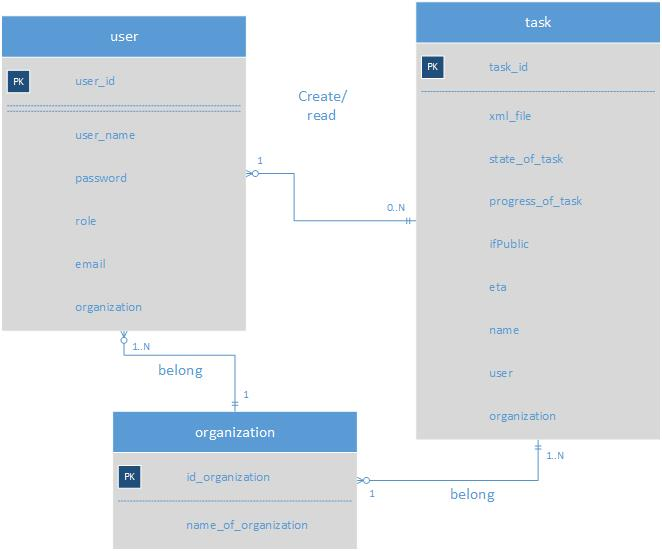
\includegraphics[scale=0.5]{ER.jpg} 
\caption{ER diagram}
\label{ER}

\end{center}

\end{figure}

Tento obrázok zobrazuje jednotlivé entity, ktoré sú potrebné na uloženie v databáze, každá z nich ma určité položky. ER diagrama sa skladá z 3 entít: user - entita, ktorá reprezentuje užívateľ, task - entita, ktorá reprezentuje úlohu a organization - entita, ktorá reprezentuje organizáciu. Výsledný návrh odpovedá skutočnosti, že každý užívateľ musí byť súčašťou organizácia, rovnako môže mať vytvorené 0 až N úloh. Taktiež pre zjednodušenie je každa úloha priradená priamo organizácií pre zlepšenie rýchlosti získania výsledkou a zjednodušenia ich nájdenia. Každá entita obsahuje primárny kľúč(jedná sa o silné entitné množiny), ktorý je odvodený od názvu a začína predponou \uv{id\_} a pokračuje názvom entity. Poďme sa pozrieť bližšie na jednotlivé entity. Entitná množina organization obsahuje 2 položky jednou z nich je primárny klúč a ďalšou názov organizácia podľa, ktorej sú zaraďovaný jednotlivý užívatelia. Ďalej prejdime k entitnej množine user. Táto entita má rovnako primárny kľúč. Ďalej obsahuje položku pre užívateľské meno(user\_name), heslo(password), email, užívateľskú rolu(role) a cudzí kľúcč organization, ktorý obsahuje na organizáciu. Nakoniec prejdime k entitnej množine task. Táto entitná množina obsahuje primárny kľúč, ďalej obsahuje xml súbor, ktorý reprezentuje danú úlohu(v našom prípade N dám), stav úloh(state\_of\_task, ktorý reprezentuje rôzne stavy úlohy), ktorý si podrobnejšie rozobereme. Úloha sa môže nachádzať v jednom z nasledujúcich stavov:
\begin{itemize}
\item NEW - úloha bola vytvorená
\item MODIFIED - xml súbor bol modifikovaný
\item WAITING - úloha čaká na spracovanie
\item IN\_PROGRESS - práve prebieha výpočet
\item PAUSED - úloha je pozastavená
\item COMPLETE - úloha je dokončená
\end{itemize}
Entitná množina task ďalej obsahuje položku, ktorá percentuálne hodnotí stav výpočtu úlohy(progress\_of\_task), čas do skončenia výpočtu úlohy(eta), nastavenie úlohy na privátnu alebo verejnú(ifPublic), názov úlohy(name) a cudzie kľúce user, ktorý odkazuje na užívateľa, ktorým bola úloha vytvorená a organization, ktorá odkazuje na organizáciu užívateľa, ktorým bola vytvorená. V ďalšej kapitole sa pozrieme na use case diagram.



\subsection{Diagram užitia}
Nasledujúci obrázok ukazuje príprady užitia systému:
\begin{figure}[htb]

\begin{center}

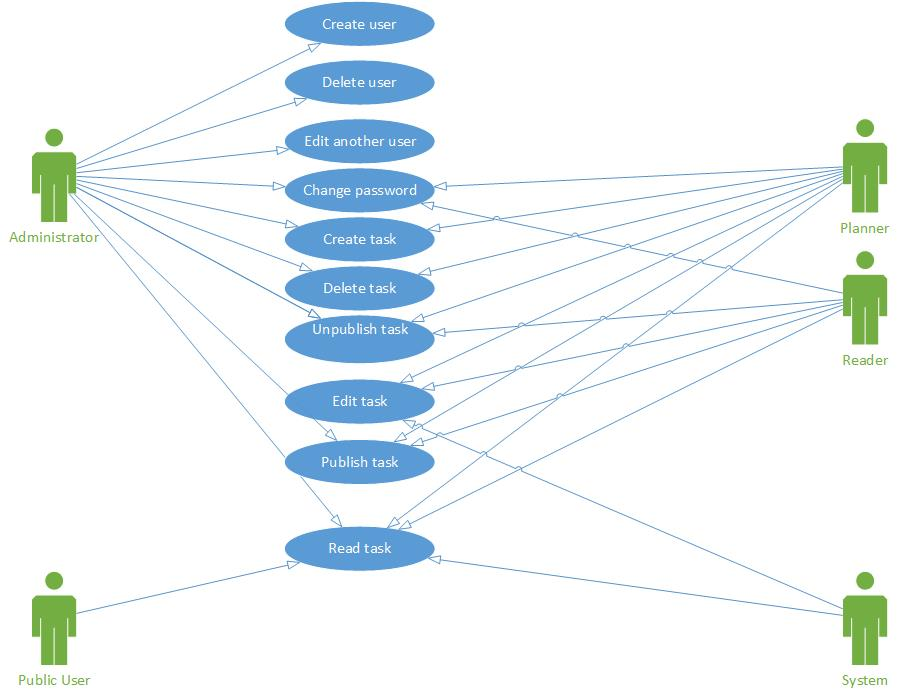
\includegraphics[scale=0.5]{UseCase.jpg} 
\caption{UseCase diagram}
\label{use}

\end{center}

\end{figure}
Na nasledujúcom obrázku č.\ref{use} môžme identifikovať 4 užívateľov systém. Public user je verejný úžívateľ, ktorý môže čítať úlohy, ktoré sú nastavené ako verejné(public). Systém môže načítať úlohy z databáze pre potreby výpočtu, z ktorými následne pracuje, a potom výsledky ukladá do databáze, teda edituje úlohy(tasky). Čitateľ(Reader) môže úlohy čítať, publikovať a odpublikovať. Plánovač môže úlohy čítať, vytvárať v databáze, mazať, editovať už vytvorené úlohy v rámci svojej organizácie,publikovať a odpublikovať úlohy a meniť vlastné heslo. Administrátor môže vytvárať úlohy, mazať úlohy , editovať úlohy, publikovať a odpublikovať úlohy. Rovnako si môže meniť heslo, vytvárať,mazať editovať organizácie a užívateľov.




\section{Návrh rozhrania}
Výsledné rozhranie kladie dôraz na jednoduchosť a prehľadnosť zobrazených úloh. Z tôhto dôvodu boli implementované mechanizmy vyhľadávanie úloh, organizácií a užívateľov. Rovnako možnosti lexikografického triedenia. Po prihlásení do systému Jednotlivé môžnosti sú následe zakompotované do záložiek, v ktorých je sprístupné príslušná funkčnosť. Výsledné rozhranie je prenositeľné aj na mobilné zaradenie, čo je spôsobené použitím frameworku Twitter Boostrap.


\section{Implementácie}
Aplikácie bola rozložená do viacerých tried podľa zodpovednosti daných komponent. Pri implementácií bolo použité JBoss Developer studo 7.1.1 GA spolu s JBoss AS 7.1.1 Final. Celý projekt boli založený na technológií maven, ktorú uľahčovala celý process vývoja a jeho následne nasadenie na JBoss server. Pre databázovú technológiu bol nainštalovaný mysql server nakonfigurovaný s príslunými prihlasovacími údajmi. Celý vývoj začal tvorbou balíka pre entitné triedy, ktoré pristupovali k databázami. Vývoj ďalej pokračoval tvorbou triedy, ktorá implementuje všetky potrebné operácie nad dátami. Následne treba správne nakonfigurovať datasource v JBoss AS, aby mohol správne pristupovať k databázmi vrátane prihlasovacích údajov. Následne pre správne priprájanie nasadeného maven projektu trebalo nastaviť súbor persistence.xml, do ktorého sa definovali entitné triedy a odkaz na datasource umiestneného na JBoss AS. Následne som sa sústredil na vývoj samotného užívatelského rozhrania. Užívateľské rozhranie som rozdelil do do 4 Managed bean, ktoré sa starajú o funkčnosť implementovaných xhtml stránok. Stránky sú celkom 4 , 3 pre užívatelské role, 4. pre prihlasovanie do systému. Každej stránke pritom odpovedá managed beana. Prihlasovacia stránka je upravená prostredníctvom Twitter Bootstrap-u, pričom obsahuje zabezpečenie prostredníctvom uživatelských rol. Rovnako obsahuje validáciu pred nekorektným prihlasovaním, ktoré môže byť spôsobené neznámym užívateľským meno alebo heslom. Následne je užívateľ presmerovaný na základe svojej role na príslušnú stránka. Každá stránka obsahuje záložky a podla svojej role dovodluje užívatelia vykonávať akcie. Základom každého zobrazenie je dátová tabulka h:datatable, ktorá zodpovedá príslušnému modelu(užívateľ, úloha, organizácia s príslušnými vlastnosťami), ktorá zobrazuje údaje na stránku a neustále obnovuje svoj obsah podľa obsahu v databázi. Príslušné riadky odpovedajú položkám v databázi pričom pre každú položku sa vzťahuje nejaká akcia, ktorá je reprezentovaná prislušným tlačidlom. Po stlačení tlačidla sa prislušna zmena prejaví na stránke rovnako ako aj na stránke. Vytváranie novej úlohy je reprezentované komponentov rich:upload, ktorá pochádza z frameworku Rich Faces. Táto komponenta zabezpečuje nahrávanie xml súborov, ktoré reprezentujú danú úlohu, celé je to zaobalené do formuláru, ktorý obsahuje položku na zadanie mena. Po stlačení tlačidla \uv{Create Task}, dôjde k zavolaniu methódy z managed beany príslušnej triedy, ktorá sa postará o vytvorenie úlohy v databázi a jej zobrazenie na stránke. V každú tabulku je možné zoraďovať podľa stĺpcov, deje sa to kliknutím na príslušný stĺpec, to spôsobí zavolanie metódy v managed bean-e, ktorá prejde všetky položky daného stĺpca, ktoré sú uložené v zozname a zoradí ich podľa stĺpcov. Obnovanie obsahuje sa realizuje prostredníctvom komponenty aj4:poll, ktorá je súčasťou frameworku Rich Faces. Táto komponenta neustála volá metódu, ktorá získava všetky položky z databáze, čím je zabezpečený aktuálny obsah tabuliek. Vyhľadávanie položiek v danej tabulke sa deje prostredníctvom formulára, do ktorého sa zadá vyhľadávaný reťazec a zvolí sa z vyskakovacie zoznamu, následna sa zavolá metóda, ktorá nastaví obsah h:datable na nájdené položky. Tento postup je rovnaký pre manažovanie organizácií a užívateĺov. Jednotlivé možnosti sú zakomponované od záložiek, ktoré sú implementované prostredníctvom twitter boostrap-u. Jednotlivé metódy sú pritom identické vo všetkých managed bean podľa užívatelskej role, až na to, že sú obmedzené podľa užívatelské role. Spustenie výpočtu sa deje prostredníctvom tlačidla \uv{Run Task}, to zavolé metódu \uv{Run Task} web service prostredníctvom http protokolu a predá mu ako parameter ID úlohy, ktorú má spustiť. Tá následne získa data z databáze a zaradí úlohu do fronty. Z fronty si odoberajú enterprise beany, ktoré sa môžu nachádzať kvôli rozprestrenie záťaže na viac serveroch. Tie si úlohu vyberú z actiemsq fronty a spustia výpočet. Priebežne pritom ukladajú údaje o stavu úlohy, času do ukončenia úlohy a percentuálnom ohodnotení úlohy. Po ukončení úlohy je uložené najlepšie možné riešenie do databáze. Užívateľ môže úlohy pozastaviť a to po stlačení tlačidla \uv{Stop Task}, ktoré zavolá metódu web service prostredníctvom protokolu http. Následne je možné úlohu opäť spustiť. Výsledky spracovania sú priebežne zobrazované(každé 2 sekundy) na užívateľské rozhranie. Rozhranie obsahuje validáciu, ktorá kontroluje všetky užívateľské vstupy.



\section{Testovanie}
Testovanie prebiehalo na servery JBoss AS 7.1.1 Final najprv prostredníctvom jednodúch JUnit testov, ktoré malo overiť komplikovanú fukčnosť metód. Následne sa pre overenie fukčnosti databáze použil framework Arqullian, ktorý umožňuje nasadenie tried priamo do Java EE kontajneru, čo zjednodušuje testovanie. Prostredníctvom tohto frameworku sa testovala celková fukčnosť aplikácie.

V ďalšej častie prebiehalo testovanie medzi konkrétnymi užívateľmi. Užívatelia testovali aplikáciu a hľadali buggy, ktoré neodhalilo predošlé testovanie.




\section{Vyhodnotenie aplikácie}
Po testovacej fáze nasledovala fáza vyhodnotenia aplikácie. Cielovým užívatelom bol poskytnutý prístup k aplikácií. Následne po vyskúšaní aplikácie vyplnili dotáznik, ktorá poskytoval celkový pohľad na aplikáciu.


















\chapter{Záver}



